\documentclass[titlepage,landscape]{seminar}
\usepackage{url}
\usepackage{graphicx}
\usepackage[pdftex]{color}
\usepackage{hyperref}
\usepackage{epstopdf}
\usepackage{slides}

\newcommand{\frack}{\frac{1}{k}}

\begin{document}

\myslide{
\begin{eqnarray*}
\hat x_{11} &=& p^2 + fpq \\
\hat x_{12} &=& 2pq(1-f) \\
\hat x_{22} &=& q^2 + fpq
\end{eqnarray*}
}

\myslide{
\begin{center}
\begin{tabular}{rcccc}
Identity by descent \\
      &            & $A_1$ & $\rightarrow$ & $A_1$ \\
      & $\nearrow$ &       &               & \\
$A_1$ &            &       &               & \\
      & $\searrow$ &       &               & \\
      &            & $A_1$ & $\rightarrow$ & $A_1$ 
\end{tabular}
\end{center}
}

\myslide{
\begin{center}
\begin{tabular}{rcccc}
Identity by type \\
      &            & $A_1$ & $\rightarrow$ & $A_1$ \\
      & $\nearrow$ &       &               & \\
$A_1$ &            &       &               & \\
      & $\searrow$ &       &               & \\
      &            & $A_2$ & $\rightarrow$ & $A_1$ \\
      & $\uparrow$ &       & $\uparrow$    & \\
      & mutation   &       & mutation      & 
\end{tabular}
\end{center}
}

\myslide{
\begin{eqnarray*}
x_{11} &=& p^2(1-f) + fp \\
x_{12} &=& 2pq(1-f) \\
x_{22} &=& q^2(1-f) + fq 
\end{eqnarray*}
\begin{eqnarray*}
x_{11} &=& p^2 + fpq \\
x_{12} &=& 2pq(1-f) \\
x_{22} &=& q^2 + fpq 
\end{eqnarray*}
}

\myslide{
\begin{center}
\begin{tabular}{l|rrr}
\hline\hline
       & $A_1A_1$ & $A_1A_2$ & $A_2A_2$ \\
\hline
From forest & 16  & 48       & 36 \\
From meadow & 49  & 42       & 9 \\
\hline
Total       & 65  & 90       & 45 \\
\hline
\end{tabular}
\end{center}

\begin{eqnarray*}
p &=& \frac{2(65) + 90}{2(65 + 90 + 45)} \\ 
  &=& 0.55 \\
  &=& 0.5(0.4 + 0.7)
\end{eqnarray*}
}

\myslide{
\begin{center}
\begin{tabular}{l|rrr}
\hline\hline
       & $A_1A_1$ & $A_1A_2$ & $A_2A_2$ \\
\hline
From forest & 16  & 48       & 36 \\
From meadow & 49  & 42       & 9 \\
\hline
Total       & 65  & 90       & 45 \\
Expected (from $p=0.55$)    & (0.3025)200 & (0.4950)200 & (0.2025)200 \\
                            & 60.5     & 99.0     & 40.5 \\
\hline
\end{tabular}
\end{center}
}

\myslide{
\begin{center}
\begin{tabular}{l|rrr}
\hline\hline
         & $A_1A_1$       & $A_1A_2$         & $A_2A_2$ \\
\hline
Expected & $\bar p^2$     & $2\bar p\bar q$  & $\bar q^2$ \\
Observed & $\frack\sum p_i^2$ & $\frack\sum 2p_iq_i$ & $\frack\sum q_i^2$ \\
\hline
\end{tabular}
\end{center}
}

\myslide{
\begin{eqnarray*}
\frack\sum p_i^2 &=& \frack\sum (p_i - \bar p + \bar p)^2 \\
&=& \frack\sum \left((p_i - \bar p)^2 + 2\bar p(p_i - \bar p)
                            + \bar p^2\right) \\
             &=& \frack\sum (p_i - \bar p)^2 + \bar p^2 \\
             &=& \hbox{Var}(p) + \bar p^2 \label{eq:p2} \\
\frack\sum 2p_iq_i &=& 2\bar p\bar q - 2\hbox{Var}(p) \label{eq:2pq} \\
\frack\sum q_i^2   &=& \bar q^2 + \hbox{Var}(p) \label{eq:q2}
\end{eqnarray*}
}

\myslide{
\begin{center}
\begin{tabular}{l|rcrcr}
\hline\hline
         & Expected &   &           &   & Observed \\
\hline
$A_1A_1$ &   0.3025 & + &   0.0225  & = &   0.3250 \\
$A_1A_2$ &   0.4950 & - & 2(0.0225) & = &   0.4500 \\
$A_2A_2$ &   0.2025 & + &   0.0225  & = &   0.2250 \\
\hline
\end{tabular}
\end{center}
}

\myslide{
\begin{eqnarray*}
\frack\sum p_i^2 &=& \bar p^2 + F_{st}\bar p \bar q \label{eq:p2-f} \\
\frack\sum 2p_iq_i &=& 2\bar p\bar q(1 - F_{st}) \label{eq:2pq-f} \\
\frack\sum q_i^2   &=& \bar q^2 + F_{st}\bar p \bar q \label{eq:q2-f}
\end{eqnarray*}
}

\myslide{
\[
F_{it} = 1 - \frac{H_i}{H_t}
\]
\begin{eqnarray*}
1 - F_{it} &=& \frac{H_i}{H_t} \\
           &=& \left(\frac{H_i}{H_s}\right)\left(\frac{H_s}{H_t}\right) \\
           &=& (1 - F_{is})(1 - F_{st}) 
\end{eqnarray*}
}

\myslide{
\begin{center}
\begin{tabular}{c|rrr|c}
\hline\hline
           & \multicolumn{3}{c|}{Genotype} & \\
Population & $A_{1}A_{1}$ & $A_{1}A_{2}$ & $A_{2}A_{2}$ & $\hat p$ \\
\hline
Yackeyackine Soak     & 29 & 0 & 0 & 1.0000 \\
Gnarlbine Rock        & 14 & 3 & 3 & 0.7750 \\
Boorabbin             & 15 & 2 & 3 & 0.8000 \\
Bullabulling          & 9  & 0 & 0 & 1.0000 \\
Mt. Caudan            & 9  & 0 & 0 & 1.0000 \\
Victoria Rock         & 23 & 5 & 2 & 0.8500 \\
Yellowdine            & 23 & 3 & 4 & 0.8167 \\
Wargangering          & 29 & 3 & 1 & 0.9242 \\
Wagga Rock            & 5  & 0 & 0 & 1.0000 \\
``Iron Knob Major''   & 1  & 0 & 0 & 1.0000 \\
Rainy Rocks           & 0  & 1 & 0 & 0.5000 \\
``Rainy Rocks Major'' & 1  & 0 & 0 & 1.0000 \\
\hline
\end{tabular}
\end{center}
}

\myslide{
\begin{eqnarray*}
\bar p &=& 0.8888 \\
\hbox{Var}(p) &=& 0.02118 \\
F_{st} &=& 0.2143 \\
\hbox{Individual heterozygosity} &=& 0.1340 \\
\hbox{Expected heterozygosity} &=& 0.1976 \\
F_{it} &=& 0.3221 \\
       1 - F_{it} &=& (1 - F_{is})(1 - F_{st}) \\
           F_{is} &=& 0.1372
\end{eqnarray*}
}

\myslide{
\begin{eqnarray*}
\mbox{E}(\hat p) &=& \mbox{E}\left(\sum (k/n)\right) \\
          &=& \sum (k/n) P(k) \\
          &=& (1/n)\left(\sum k P(k)\right) \\
          &=& (1/n)(n p) \\
          &=& p 
\end{eqnarray*}
}

\myslide{
\begin{eqnarray*}
\mbox{E}(\tilde H) &=& \mbox{E}\left(2\hat p (1 - \hat p)\right) \\
     &=& 2\left(\mbox{E}(\hat p) - \mbox{E}({\hat p}^2)\right) \\
     &=& \mbox{TAMO} \\
     &=& ((n-1)/n)2p(1-p) 
\end{eqnarray*}
}

\myslide{
\begin{eqnarray*}
H_{i} &=& 1 - {1 \over N} \sum_{k=1}^{N} \sum_{i=1}^{m} {X_{kii}} \\
H_{s} &=& {\tilde n \over {\tilde n - 1}}
         \left[1 - \sum_{i=1}^{m} {\bar {\hat x_{i}^{2}}} 
         - {H_{I} \over {2 \tilde n}}\right] \\
H_{t} &=& 1 - \sum_{i=1}^{m} {\bar x_{i}^{2}} + {H_{S} \over {\tilde n}}
         - {H_{I} \over {2 \tilde n N}} 
\end{eqnarray*}
\begin{eqnarray*}
F_{is} &=& 1 - {H_{i} \over H_{s}} \\
F_{st} &=& 1 - {H_{s} \over H_{t}} \\
F_{it} &=& 1 - {H_{i} \over H_{t}} \quad .
\end{eqnarray*}
}

\myslide{
\begin{center}
\begin{tabular}{c|ccc}
\hline\hline
Method & $F_{is}$ & $F_{st}$ & $F_{it}$ \\
\hline
Direct            & 0.1372 & 0.2143 & 0.3221 \\
Nei               & 0.3092 & 0.2395 & 0.4746 \\
Weir \& Cockerham & 0.5398 & 0.0387 & 0.5577 \\
\hline
\end{tabular}
\end{center}
}

\myslide{
\begin{eqnarray*}
n_{11,i} &=& \hbox{\# of $A_1A_1$ genotypes} \\
n_{12,i} &=& \hbox{\# of $A_1A_2$ genotypes} \\
n_{22,i} &=& \hbox{\# of $A_2A_2$ genotypes} \\
i         &=& \hbox{population index} \\
I         &=& \hbox{number of populations} \\
\end{eqnarray*}
\begin{eqnarray*}
x_{11,i} &=& p_{i}^2 + fp_{i}(1-p_{i}) \\
x_{12,i} &=& 2p_{i}(1-p_{i})(1-f) \\
x_{22,i} &=& (1-p_{i})^2 + fp_{i}(1-p_{i})
\end{eqnarray*}
}

\myslide{
\[
P({\bf n}|{\bf p},f) \propto \prod_{i=1}^I x_{11,i}^{n_{11,i}}
x_{12,i}^{n_{12,i}} x_{22,i}^{n_{22,i}}
\]
\begin{eqnarray*}
\mbox{E}(p_{ik}) &=& \pi \\
\mbox{Var}(p_{ik}) &=& \pi(1-\pi)\theta
\end{eqnarray*}
}

\myslide{
\resizebox{0.8\textwidth}{!}{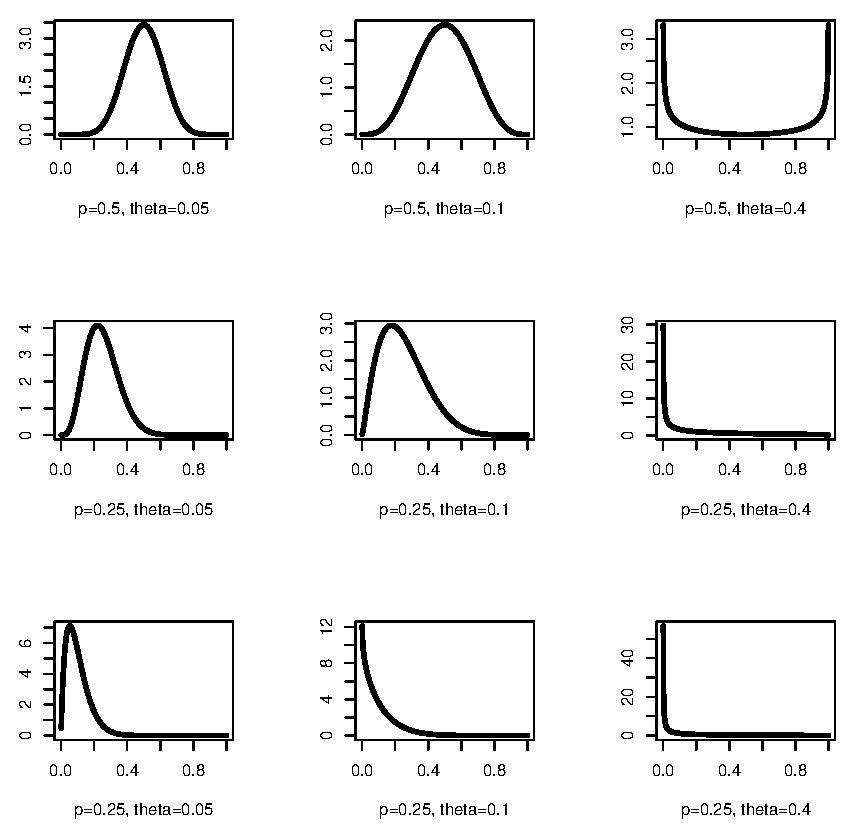
\includegraphics{beta-distribution.eps}}
}

\myslide{
\begin{center}
\begin{tabular}{cccc}
\hline\hline
           &             & \multicolumn{2}{c}{Credible Interval} \\
Parameter  & Mean (s.d.)     & 2.5\% & 97.5\% \\
\hline
$f$            & 0.52 (0.10) & 0.32 & 0.70 \\
$\theta$ & 0.19 (0.12) & 0.03 & 0.50 \\
$G_{st}^B$      & 0.10 (0.07) & 0.02 & 0.30 \\
\hline
\end{tabular}
\end{center}
}

\myslide{
\begin{center}
\begin{tabular}{l|rrrr}
\hline\hline
Model & {\tt Dbar} & {\tt Dhat} & {\tt pD} & {\tt DIC} \\
\hline
Full  & 46.5 & 40.7 & 5.8 & 52.3 \\
$f=0$ & 73.0 & 67.6 & 5.3 & 73.8 \\
$\theta=0$ & 61.6 & 59.8 & 1.8 & 63.5 \\
\hline
\end{tabular}
\end{center}
}

\myslide{
\begin{center}
\begin{tabular}{c|ccc}
\hline\hline
Method & $F_{is}$ & $F_{st}$ \\
\hline
Direct            & 0.14 & 0.21 & 0.32 \\
Nei               & 0.31 & 0.24 & 0.47 \\
Weir \& Cockerham & 0.54 & 0.04 & 0.56 \\
Bayesian          & 0.53 (0.33, 0.70) & 0.11 (0.02, 0.22) \\
\hline
\end{tabular}
\end{center}
}

\end{document}



\end{document}

